\chapter{Introduction and Motivation}

%Motivated by the recent surge in income inequality in Australia, this study seeks to explore the relationship between employee income and technical change. We perform an empirical investigation, first of the `canonical' neoclassical model of skill-biased technical change. We show that skill bias does not explain the observed empirical regularities in the wage distribution. We show that, instead, models of the task content of workers' skills, of the type proposed by \citet{Levy2003}, go some way to explaining the changing remuneration patterns of the Australian workforce.

The second half of the 20th century has witnessed tremendous change for Australian workers. To a great extent, these changes reflect the beneficial effect of economic growth: since 1973, average real per capita incomes have approximately doubled, and economic growth has added over three million jobs to the work force \citep{ABS5206,LFSApr2013}. Yet, even as mean incomes have increased and the work force expanded, these benefits have been unevenly spread. The period bore witness to a dramatic change in the distribution of incomes: Australia, like many developed countries, became less equal. After falling for the four decades following the Second World War, from the 1980s the gap between high and low income earners grew sharply, a period \citet{Leigh2013} calls the `Great Divergence.' During this time, top percentile wage earners saw their incomes increase dramatically, whereas some groups of workers did not see much income growth at all \citep{Atkinson1997,Borland1999,Leigh2013}.

The motivation for studying the changing determinants of income is perhaps obvious. To the extent that an individual's welfare is determined by the resources at his or her disposal, understanding those factors that drive changes in the level and distribution of wealth is an important role for the social sciences. To properly analyze wealth inequality, the determinants of household income flows need to be understood. However, the sheer diversity of these flows complicates this task. Household wealth can be accumulated from many sources: wages from labour, dividends from financial investments, government entitlements, other lump-sum cash transfers, capital gains on assets, and so on. The scope of these study is limited to just one of these flows: wages from labour income. Indeed, wages are the principal source of income for the majority of Australian households. Thus, any changes to the distribution of labor income are likely to have a significant impact on households' welfare. 

%A somewhat less obvious application of an understanding of the ever-shifting wage distribution, applies to education policy. Young people must choose educational path to equip them for a career. Neoclassical model of human capital tells us that individuals make education investment decisions with a view to their lifetime earnings. But this implies a good knowledge the returns that occupations will yield over the coming decades.

By focussing on individuals' wages, as the flow of labour income, we limit our ability to make direct inferences about welfare. Social welfare, as a function of income, is best considered at the household level, since income and housing costs are typically pooled between household members, and individuals do not spend their entire lives earning income \citep{Richardson1999,Borland1999}. Children and retirees who are not working, for example, are not directly affected by changes in the distribution of wage income, but they may experience indirect effects through the earnings of the family breadwinners. Further, because households may have multiple wage earners, evidence of growing wage inequality may not translate directly into income inequality between households. \citet{Richardson1999} provide evidence that individuals earning very low incomes are more likely to work part-time, as a secondary source of household income. Indeed, individuals may actually prefer to accept low-wage, part-time work, rather than higher-paid work that carries a greater time burden. Notwithstanding these limitations, in this study we consider changes in the distribution of income earned as an employee.

\begin{figure}[h]
  \centering
  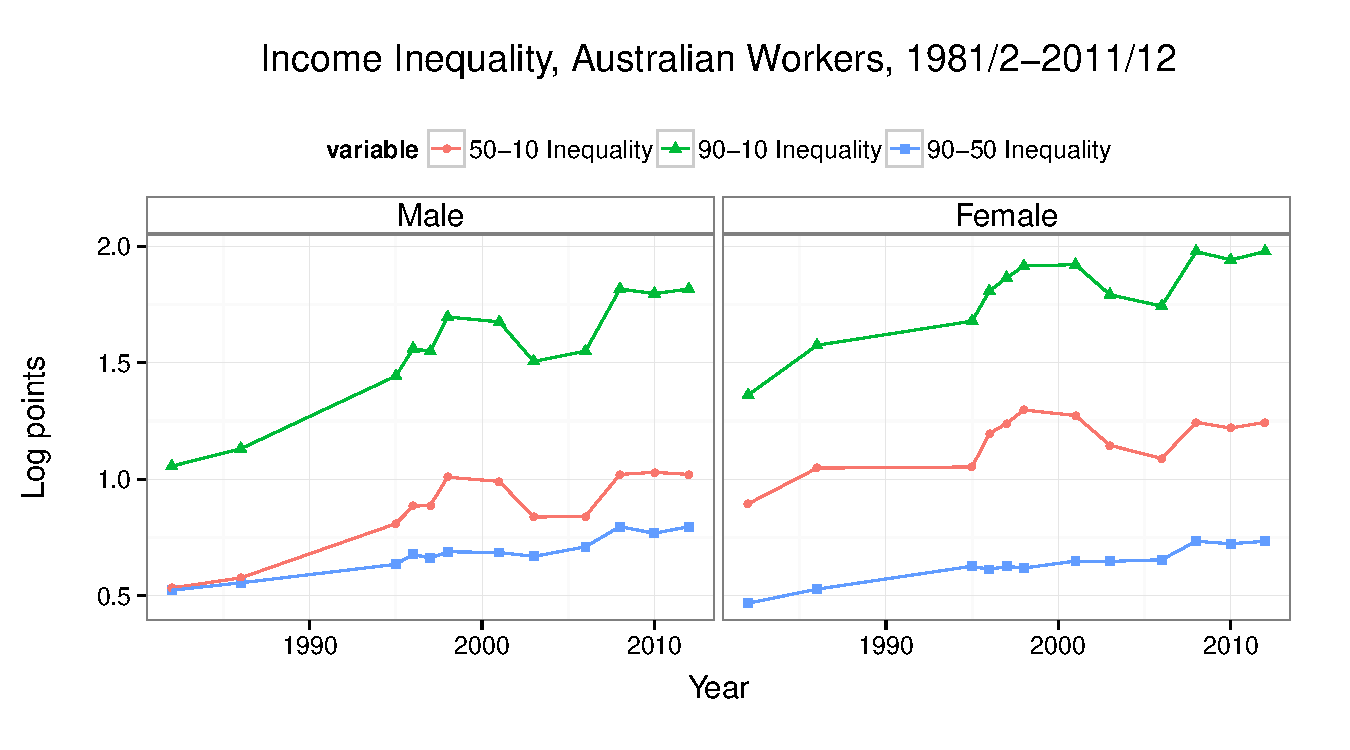
\includegraphics[width=\textwidth]{../figure/ineq_time.pdf}
  \caption{Change in income inequality measures for Australian workers, 1981/82 to 2011/12. The three measures refer to the differences between deciles of the log wage distribution. Unlike subsequent chapters of this study, which considers only full-time workers, these calculations include part-time as well as full-time employees, and workers of own account. Working populations are composition adjusted according to four educational attainment levels and five age categories. All calculations are weighted by survey weight. Source: ABS cat. 6543.0, 6541.0, 6503.0.}
\end{figure}

Understood as the dispersion of wage income earned by Australian workers, income inequality has grown over the period of the `Great Divergence' in Australia. Figure~\ref{fig:ineq} illustrates three measures of wage inequality, computed as the gap between quantiles of the log earnings distribution. {\em 90-10 inequality}, the difference between the 90th and 10th quantiles, summarizes the overall spread of the earnings distribution. {\em 90-50} and {\em 50-10 inequality} respectively describe the extent of the upper and lower `tails' of the distribution, relative to the median. Over the 30 years since the 1981/82 fiscal year and 2011/12, 90-10 inequality grew from 1.1 to 1.8 log points for males, and from 1.3 to 2.0 log points for females. In percentage terms, the income gap between men earning at the 90th percentile has grown from about 200\% of incomes of men in the 10th percentile, to about 300\% in 2011/12. For women, this figure has grown from 267\% to 639\%.

% compare this to overseas numbers

The causes of this rapid increase in income inequality in Australia have been the subject of some debate, and it is unlikely to be the outcome of any single change of labor market conditions. \citet{Leigh2013} names three principal causes for this surge in income inequality in Australia: falling union rates, falling income taxes and skill-biased technology. 

The relationship between the rate of union membership and inequality has been well-established (see, {\em inter alia}, \cite{Borland1996}).  Unions tend to reduce income inequality in the bottom of the income distribution, because they tend to bargain for across-the-board wage agreements rather than individually-negotiated employment contracts, resulting in a `compression' of the income distribution. Unions have also argued for limitations on top executive pay \citep{Davis2009}. Any reduction in the rate of union membership therefore limits the degree of wage compression, so magnifying income inequality. This effect has been well studied elsewhere: empirical studies in the US, UK and Canada have found a signficantly negative union effect on inequality \citet{Card2004,Firpo2009}. 

The second major cause for Great Divergence is falling income taxation rates. The top marginal income tax rate in the 1908s was around 60 per cent, but this has fallen to around 40 per cent today. Consequently, the average tax rate paid by wealthy Australians has fallen, resulting in a greater divergence of accumulated wealth across the population \citet[p31]{Leigh2013}. \citet{Atkinson2013} estimate that about one third of the increase in inequality in top incomes is due to decreases in income tax.

But by far the greatest driver of increasing inequality is the inexorable rise in workplace technology. In particular, new computer and information technologies disproportionately complements skilled workers making them much more productive, but leaving unskilled workers' productivity largely unchanged. Under this model of so-called `skill biased technical change' (SBTC), new workplace technologies disproportionately complement highly-skilled technical and managerial labour \citep{Griliches1969,Autor2006}. As a result of higher productivity, wages for high-skilled jobs increase, with demand for workers outstripping the supply. Likewise, as the relative demand for lower-skilled workers has softened, so relative wage growth has stagnated. 

The three phenomena outlined above may not operate independently. \citet{Acemoglu2003} analyze a model where skill-biased technology reduces the incentives for workers to accept the trade-off between lower wages and the improved job security and bargaining services that unions offer. If skill-biased technology improves the earnings capacity for workers with higher levels of talent or human capital, then the opportunity cost of giving up individually-negotiated contracts (where earnings may depend on that indvidual's above-average level of productivity) is considerably higher. It is thus possible that unions `amplify' inequality caused by skill-baised technical change.

The surge in inequality over the past 30 years is not a uniquely Australian experience. \citet{Atkinson2013} analyze top income rates from five Anglo-Saxon countries' tax data, and find that Australian trends described above correspond closely to the inequality patterns seen in the US, UK, Canada and New Zealand, on a wide variety of inequality measures. In all five countries, the income share accruing to the richest 0.1 per cent of income earners fell over the middle part of the twentieth century. In 1920, this group received between four and six per cent of national income (eight per cent in the U.K.), a figure that was to fall over the following half century to a nadir of around two per cent in 1980. Since the 1980s, the so-called Great Divergence has been experienced by all five countries. 

Of the many drivers of inequality, this thesis will focus on just one: the rise of skill-biased technology, and the impact of its adoption by firms. The SBTC argument, which has sparked a voluminous literature, has enjoyed considerable empirical success explaining rising wages for high-skill managerial and professional jobs in the United States and Europe \citep{Katz1992}. Since the canonical model includes \emph{factor-augmenting} capital, it predicts monotone skill upgrading of the work force at all education levels \citep{Levy2003}. Skill upgrading has been confirmed by a number of authors, both in Australia \citep{Esposto2012, Wooden2000, Cully1999} and overseas \citep{Autor2008}. 

There are good reasons for focusing on technology as a driver of changes in the work force. Although mechanical computers and computation aids (the abacus, for instance), have been available for centuries, it was only in the post-war era, with the arrival of electronic computation, that the price of computation began to fall dramatically. \citet{Nordhaus2007} estimates that, between 1946 and 2006, the cost per computation decreased by a factor of {\em seven trillion,} and over the same period, the cost of data storage fell at a comparable rate. The falling cost of computation opened up new avenues for research in information technology, so that even as computation became cheaper, new and improved algorithms were developed which made more efficient use of, and found novel uses for, computing power. And as computers have become cheaper and more useful, firms have made greater use of them. Between 1981 and 2012, Australian firms' real annual investment in computers has grown from \$26M to \$14B, in constant 2012 dollars \citet{ABS5206}.

The canonical model also predicts a rising premium for high-skill workers. In the United States in particular, SBTC has been able to explain the dynamics of the wage premium demanded by tertiary-educated labor, which fell in the 1970s and has risen in the decades to 2008 \citep{Acemoglu2011}. However, the model substantially \emph{over-predicts} the magnitude of this differential for the United States \citep{Autor2008}. In Australia, a corresponding growth in the premium for tertiary qualifications has not been observed \citep{Coelli2009}.

In addition to the lack of an observed skill premium in Australia, evidence from foreign labor markets suggests that there are a number of empirical regularities that the canonical model fails to explain. Since the late 1990s, both in Europe and the United States, the data show a marked polarization in the work force \citep{Goos2007, Autor2006}. This polarization has simultaneously manifested in \emph{wages} and in \emph{jobs}: both wage growth and growth in the level of employment are concentrated in high-skill jobs, to a lesser extent, the bottom end of the skill spectrum. Middle-skill jobs have stagnated since the 1990s, both in terms of remuneration and level.

The rise of inequality in Australia has been well documented. Empirical studies have confirmed that both individual-level and household-level inequality have been rising since the 1980s \citep{Borland1999,Leigh2005,Leigh2013,Gaston2009}. A number of studies exist on the task content of Australian jobs \citep{Esposto2012a}, and the change over time of the skill intensity of various professions \citep{Esposto2012, Esposto2012a}. Although ICT use and globalization have been found to (non-)Granger cause rising inequality at the aggregate level \citep{Gaston2009}, no studies have tested whether workers' job types and on-the-job activities explain the nature of these changes.

This research is structured according to three related, but separate lines of inquiry. In Chapter~\ref{ch:2}, we review the emprical evidence for skill-biased technical change, and produce estimates of the skill premium for recently-relased data. In Chapter~\ref{ch:3}, we extend our analysis to consider whether the impact of SBTC is polarizing, rather than simply widening, the income distribution. And finally, in Chapter~\ref{ch:4} we seek to quantify the channels by which changes in the income distribution have occured, by  decomposing changes in the income distribution into the tasks that comprise occupations. Finally, in Chapter~\ref{ch:5}, we review and suggest avenues for further research.

%%% Local Variables: 
%%% mode: latex
%%% TeX-master: "thesis"
%%% End: 
